\section{Introduction}
\label{sec:intro}

Outlier-robust point cloud registration is a fundamental and long-studied problem, it is the core of many applications such as scene reconstruction or localization in autonomous driving. Most available methods solve the problem satisfactorily but provide no guarantees -- they are hard instances of the problem, either with many outliers (e.g. 90\%) or symmetries in the scene. On such instances, point cloud registration often fails, outputting an arbitrarily wrong solution.

From a statistical point of view, this is essentially a robust regression problem, more specifically a best-subset selection. This means, we need to find the best subset of data points as well as the model parameters that best fit this subset.
The model is in this case a rigid 3D-transformation, the model parameter a rigid transform $\in \SEthree$. Each data point is a pair of corresponding 3D points of from both point clouds.

\begin{figure}[!ht]
	\centering
	\begin{adjustbox}{width=1.\linewidth}
		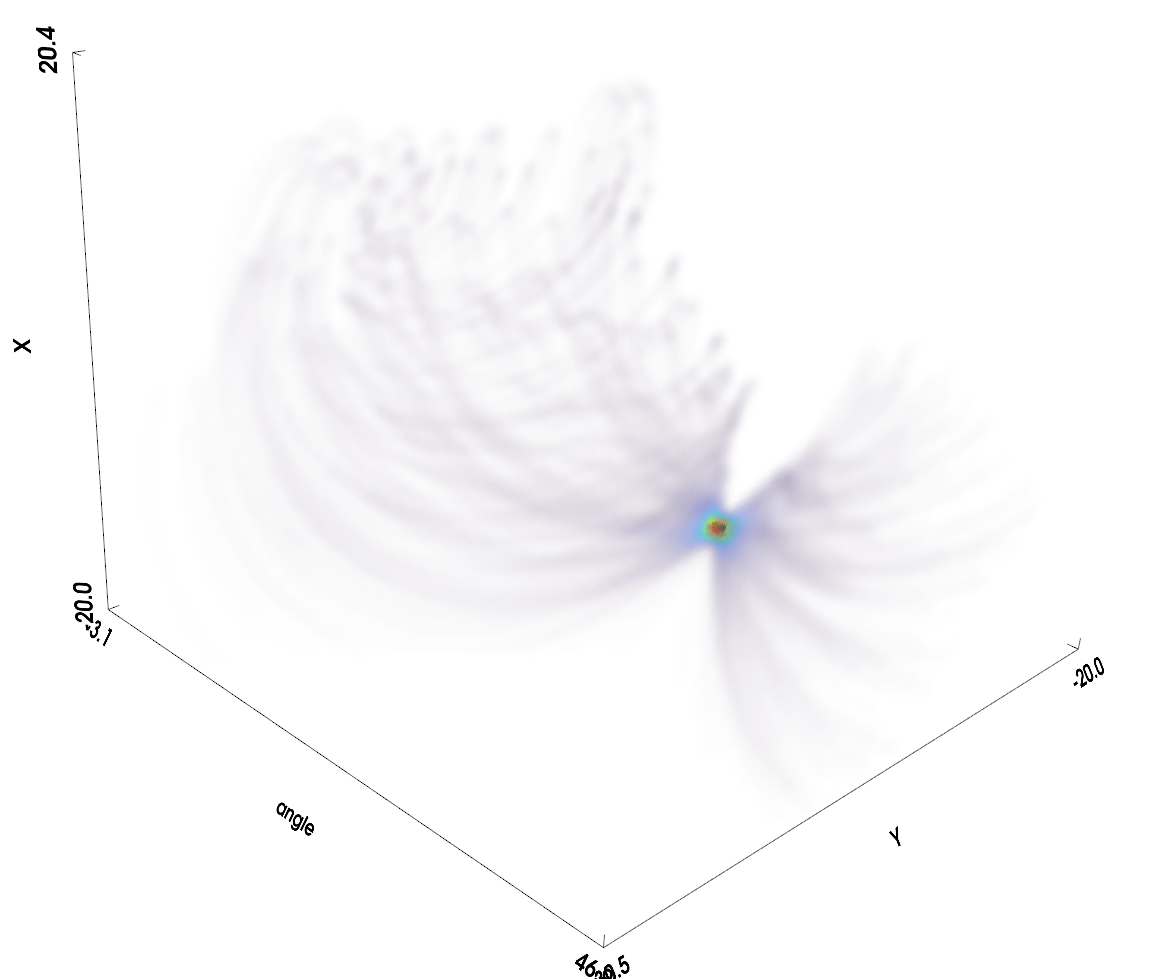
\includegraphics{figures/tls_objective_se2.png}
	\end{adjustbox}
	\caption{The Truncated Least Squares objective function over $SE(2)$ (2D point cloud registration problem)}
	\label{fig:tls-objective}
\end{figure}

In summary, our main contributions are (TODO): 
\begin{enumerate}
	\item A convex relaxation for the Truncated Least Squares objective function that can be computed in linear time
	\item Computationally very efficient custom solvers for minimizing the convex relaxation over translations and rotations
\end{enumerate}





